\documentclass[12pt,a4paper]{article}
\usepackage[a4paper,margin=1in]{geometry}
\usepackage{parskip}
\usepackage{fontspec}
\usepackage[polish]{babel}
\setmonofont{NotoSansMono-Regular.ttf}[Scale=0.82]
\usepackage{microtype,booktabs,tabularx,longtable,array,graphicx,float,caption,enumitem}
\usepackage{fvextra}
\usepackage{xcolor,tikz}
\usetikzlibrary{positioning,arrows.meta,fit}
\usepackage{xurl}
\usepackage[hidelinks]{hyperref}
\newcommand{\autor}{Damian Osiński}
\newcommand{\album}{[nr albumu]}
\newcommand{\uczelnia}{[uczelnia, wydział, kierunek]}
\newcommand{\prowadzacy}{[prowadzący]}
\newcommand{\datapracy}{listopad 2026}

\graphicspath{{img/}}
\newcommand{\kod}[1]{\texttt{#1}}
\newcommand{\vuln}{\textsc{vuln}}
\newcommand{\secure}{\textsc{secure}}
\fvset{fontsize=\footnotesize,breaklines,breakanywhere,frame=single,framesep=2mm,rulecolor=\color{gray}}
\usepackage{etoolbox}
\BeforeBeginEnvironment{Verbatim}{\par\medskip\noindent\begin{minipage}{\linewidth}}
\AfterEndEnvironment{Verbatim}{\end{minipage}\par\medskip}
\newcommand{\dowod}[3][]{\par\medskip\noindent\begin{minipage}{\linewidth}\VerbatimInput[label=#3,#1]{evidence/#2}\end{minipage}\par\medskip}
\setlist{itemsep=2pt,topsep=3pt}
\emergencystretch=2em
\newcolumntype{L}[1]{>{\raggedright\arraybackslash}p{#1}}

\begin{document}
\pagenumbering{gobble}
\begin{titlepage}
\centering
\vspace*{\fill}
{\large \uczelnia\par}
{\large \wydzial\par}
{\large \katedra\par}
\vfill
{\large \przedmiot\par}
\vspace{0.6cm}
{\LARGE\bfseries Projekt\par}
\vspace{0.35cm}
{\large Aplikacja CRUD w~wersji zabezpieczonej i~niezabezpieczonej \\ --- analiza zachowania i~ruchu sieciowego\par}
\vfill
{\large \autorzy\par}
{\large grupa \grupa\par}
\vspace{0.3cm}
{\large \today\par}
\vspace*{\fill}
\end{titlepage}

\tableofcontents
\newpage
\pagenumbering{arabic}

\section{Wstęp}

\subsection{Cel i zakres}
Celem projektu jest opracowanie prostej aplikacji CRUD oraz porównanie jej zachowania, w~tym ruchu sieciowego, w~wersji zabezpieczonej i~niezabezpieczonej. Aplikacja \emph{notes-cyber-project} jest notatnikiem wieloużytkownikowym: po zalogowaniu użytkownik tworzy, przegląda, wyszukuje, edytuje i~usuwa własne notatki.

Obie wersje powstają z~jednego kodu źródłowego. O~trybie decyduje zmienna środowiskowa \kod{SECURE}:
\begin{itemize}
\item \vuln{} (\kod{SECURE=0}) --- HTTP na porcie 3000, wszystkie zabezpieczenia wyłączone,
\item \secure{} (\kod{SECURE=1}) --- HTTPS na porcie 3443, wszystkie zabezpieczenia włączone.
\end{itemize}
Dzięki temu różnice w~wynikach pomiarów i~ataków wynikają wyłącznie z~zabezpieczeń, a~nie z~odmiennej funkcjonalności. Zademonstrowano jedenaście podatności wraz z~poprawkami.

\subsection{Założenia projektowe}
\begin{enumerate}
\item Funkcjonalność (pełny CRUD, wyszukiwanie, rejestracja, logowanie) jest taka sama w~obu trybach.
\item Każdą podatność można odtworzyć skryptem lub w~przeglądarce i~w~taki sam sposób sprawdzić, że poprawka działa.
\item Minimum zależności: jedyną biblioteką zewnętrzną jest Express. Kryptografia i~baza danych pochodzą ze standardowej biblioteki Node.js, więc każdy mechanizm obronny da się wskazać w~kodzie i~omówić.
\item Baza działa w~pamięci i~jest wypełniana od nowa przy każdym starcie, co daje powtarzalny stan początkowy.
\item Tryb \vuln{} służy wyłącznie do demonstracji na własnym komputerze; nie wolno wystawiać go do sieci.
\end{enumerate}
Poza zakresem są: wysoka dostępność, trwałość danych, atak na system operacyjny serwera i~na stację użytkownika.

\section{Przegląd literatury}

\paragraph{Klasyfikacja zagrożeń.} Punktem odniesienia jest OWASP Top~10. Wydanie z~2025~r.~\cite{owasptop10} na pierwszym miejscu umieszcza błędy kontroli dostępu (A01), następnie błędną konfigurację (A02) i~zagrożenia łańcucha dostaw oprogramowania (A03); wstrzyknięcia zajmują pozycję A05, a~nową kategorią jest niewłaściwa obsługa sytuacji wyjątkowych (A10). Wymagania szczegółowe opisuje standard ASVS~\cite{asvs}. Ogólne zasady projektowe, m.in. najmniejsze uprawnienia i~pełną mediację dostępu, sformułowali już Saltzer i~Schroeder~\cite{saltzer}.

\paragraph{Celowo podatne aplikacje.} Znanymi rozwiązaniami dydaktycznymi są DVWA, WebGoat, Juice Shop i~Gruyere. De~Roo~\cite{deroo} porównuje je pod względem pokrycia podatności, wartości dydaktycznej i~sposobu wdrożenia i~stwierdza, że żadna nie jest najlepsza w~każdym zastosowaniu. Ni~i~in.~\cite{gruyere} wykorzystują Gruyere do odtworzenia podatności z~listy OWASP oraz omówienia poprawek. Aplikacje te skupiają się na samym ataku. Niniejszy projekt uzupełnia to podejście o~działającą wersję zabezpieczoną tego samego kodu i~o~porównanie ruchu sieciowego.

\paragraph{Wstrzyknięcia SQL i~XSS.} Halfond, Viegas i~Orso~\cite{halfond} sklasyfikowali ataki SQL injection (m.in. tautologie i~zapytania UNION, oba użyte w~projekcie) oraz środki zaradcze. W~przypadku XSS dodatkową warstwą ochrony jest Content Security Policy. Weichselbaum i~in.~\cite{csp} wykazali jednak, że 94{,}68\% badanych polityk próbujących ograniczyć wykonywanie skryptów było nieskutecznych, głównie przez listy dozwolonych domen. Stąd w~projekcie polityka ograniczona do własnego źródła, bez list domen, oraz poprawne renderowanie jako zabezpieczenie podstawowe.

\paragraph{CSRF i~sesje.} Barth, Jackson i~Mitchell~\cite{barth} przeanalizowali obrony przed CSRF: tajny token, nagłówek \kod{Referer} i~nagłówki niestandardowe. Obecnie uzupełnia je atrybut \kod{SameSite}, opisany w~projekcie następcy RFC~6265~\cite{rfc6265,rfc6265bis}. OWASP~\cite{owaspsession} wymaga identyfikatora sesji o~entropii co najmniej 64~bitów, atrybutów \kod{Secure}, \kod{HttpOnly} i~\kod{SameSite} oraz wygasania sesji egzekwowanego po stronie serwera.

\paragraph{Hasła.} OWASP~\cite{owasppass} zaleca Argon2id, a~gdy jest niedostępny --- scrypt~\cite{rfc7914}. NIST SP~800-63B-4~\cite{nist} wymaga co najmniej 15~znaków, jeśli hasło jest jedynym składnikiem uwierzytelniania; ASVS~5.0 dopuszcza 8, silnie zalecając 15.

\paragraph{Ochrona transmisji.} TLS~1.3 opisuje RFC~9846~\cite{rfc9846} (lipiec 2026), który zastąpił RFC~8446. HSTS~\cite{rfc6797} zapobiega powrotowi do HTTP. RFC~10024~\cite{rfc10024} wprowadza hybrydowe, odporne na komputery kwantowe uzgadnianie klucza, m.in. X25519MLKEM768. Szyfrowanie nie ukrywa wszystkiego: Chen i~in.~\cite{chen} pokazali, że rozmiary i~kolejność zaszyfrowanych pakietów ujawniają działania użytkownika aplikacji webowej. Zjawisko to potwierdzono pomiarem w~rozdziale~\ref{sec:ruch}.

\section{Analiza i dobór technik}

Tabela~\ref{tab:dobor} zestawia decyzje projektowe, rozważane alternatywy i~uzasadnienie.

\begin{longtable}{L{2.3cm}L{3.2cm}L{2.9cm}L{5.5cm}}
\caption{Dobór technik}\label{tab:dobor}\\
\toprule
Obszar & Wybór & Alternatywy & Uzasadnienie\\
\midrule\endfirsthead
\toprule Obszar & Wybór & Alternatywy & Uzasadnienie\\ \midrule\endhead
\bottomrule\endfoot
Platforma & Node.js + Express & Django, Spring & Frameworki „z~bateriami” domyślnie włączają ochronę, która w~projekcie ma być jawna i~przełączalna.\\
Baza & SQLite w~pamięci (\kod{node:sqlite}) & PostgreSQL, ORM & Surowy SQL jest potrzebny do pokazania wstrzyknięcia; brak osobnego serwera upraszcza odtworzenie.\\
Ochrona SQL & Zapytania parametryzowane & Filtrowanie, escaping & Struktura zapytania jest ustalona przed podstawieniem danych, więc klasa błędu znika, zamiast być filtrowana.\\
XSS & \kod{textContent} + CSP & Sanitizer HTML & Notatki to zwykły tekst, HTML nie jest potrzebny. CSP jest drugą, niezależną warstwą.\\
Hasła & scrypt ($N=2^{14}$, $r=8$, $p=5$) & Argon2id, bcrypt, PBKDF2 & Funkcja dostępna w~\kod{node:crypto}, pamięciożerna, parametry z~listy OWASP~\cite{owasppass}. Domyślne $p=1$ w~Node.js jest słabsze.\\
Sesja & Losowy token 256~b w~cookie, stan na serwerze & JWT & Sesję można natychmiast unieważnić przy wylogowaniu; JWT wymagałby listy odwołań.\\
Cookie & \kod{\_\_Host-}, \kod{Secure}, \kod{HttpOnly}, \kod{SameSite=Strict} & \kod{localStorage} & Token niedostępny dla JavaScriptu; przedrostek wymusza \kod{Secure}, \kod{Path=/} i~brak \kod{Domain}.\\
CSRF & Token w~nagłówku + \kod{SameSite} & Tylko \kod{SameSite} & Same atrybuty cookie nie wystarczają --- potwierdził to test w~Firefoksie (rozdz.~\ref{sec:csrf}).\\
Brute force & 5 nieudanych prób/60~s na adres IP, kod 429 & CAPTCHA, blokada konta & Blokada konta pozwalałaby napastnikowi odciąć ofiarę. Liczone są tylko próby nieudane.\\
Transmisja & HTTPS w~Node.js, certyfikat \kod{mkcert} & Reverse proxy, self-signed & Brak dodatkowych usług; lokalne CA daje połączenie bez ostrzeżeń, jak w~produkcji.\\
Analiza ruchu & Wireshark/tshark & tcpdump, Burp & Dekodowanie HTTP i~TLS, możliwość skryptowania, deszyfrowanie za pomocą kluczy sesji.\\
\end{longtable}

\section{Projekt systemu}

\subsection{Architektura}
\begin{figure}[H]\centering
\begin{tikzpicture}[node distance=6mm and 5mm,box/.style={draw,rounded corners=2pt,align=center,font=\footnotesize,minimum height=9mm,inner sep=4pt},>={Latex}]
\node[box] (b) {Przeglądarka\\\kod{public/app.js}};
\node[box,right=24mm of b] (h) {Nagłówki\\\kod{applyHeaders}};
\node[box,right=of h] (s) {Sesja\\\kod{requireAuth}};
\node[box,right=of s] (c) {CSRF, walidacja\\\kod{requireCsrf}};
\node[box,below=10mm of c] (r) {Operacja CRUD\\\kod{server.js}};
\node[box,left=of r] (d) {SQLite\\\kod{db.js}};
\node[box,left=of d] (e) {Obsługa błędów\\\kod{errorHandler}};
\node[draw,dashed,rounded corners=3pt,fit=(h)(s)(c)(r)(d)(e),inner xsep=7pt,inner ysep=9mm,label={[font=\footnotesize]above:proces Node.js (\kod{SECURE} = 0/1)}] (p) {};
\draw[<->] (b) -- node[above,font=\scriptsize]{HTTP} node[below,font=\scriptsize]{lub TLS 1.3} (h);
\draw[->] (h) -- (s); \draw[->] (s) -- (c); \draw[->] (c) -- (r); \draw[<->] (r) -- (d); \draw[->,dashed] (r.south) -- ++(0,-4mm) -| node[pos=.25,below,font=\scriptsize]{błąd} (e.south);
\end{tikzpicture}
\caption{Przepływ żądania. Flaga \kod{SECURE} zmienia działanie wszystkich elementów poza sprawdzeniem sesji.}
\end{figure}

\begin{table}[H]\centering\caption{Struktura kodu}
\begin{tabularx}{\linewidth}{lX}
\toprule
Plik & Rola\\\midrule
\kod{server.js} & Endpointy; w~trybie \vuln{} zapytania sklejane z~tekstu i~bez kontroli właściciela\\
\kod{security.js} & Sesje, cookie, nagłówki, CSRF, limit logowań, walidacja, obsługa błędów\\
\kod{db.js} & Schemat, dane początkowe, haszowanie i~weryfikacja haseł\\
\kod{public/} & Interfejs; \kod{innerHTML} (\vuln) lub \kod{textContent} (\secure)\\
\kod{attacks/} & Skrypty i~strony ataków\\
\kod{test.js} & Automatyczne testy wszystkich podatności w~obu trybach\\
\kod{report/collect.sh} & Odtworzenie wszystkich pomiarów z~tego raportu\\
\bottomrule
\end{tabularx}
\end{table}

\subsection{Model danych i API}
Baza ma dwie tabele: \kod{users(id, username, password)} oraz \kod{notes(id, user\_id, title, body)}. Kolumna \kod{password} zawiera tekst jawny (\vuln) albo \kod{sól:skrót} (\secure).

\begin{table}[H]\centering\caption{Interfejs HTTP}
\begin{tabular}{llcc}
\toprule
Operacja & Endpoint & Sesja & Token CSRF\\\midrule
Rejestracja & \kod{POST /api/register} & & \\
Logowanie & \kod{POST /api/login} & & \\
Wylogowanie & \kod{POST /api/logout} & tak & tak\\
Bieżąca sesja & \kod{GET /api/me} & tak & \\
Lista, wyszukiwanie (R) & \kod{GET /api/notes[?q=]} & tak & \\
Odczyt (R) & \kod{GET /api/notes/:id} & tak & \\
Utworzenie (C) & \kod{POST /api/notes} & tak & tak\\
Edycja (U) & \kod{PUT /api/notes/:id} & tak & tak\\
Usunięcie (D) & \kod{DELETE /api/notes/:id} & tak & tak\\
\bottomrule
\end{tabular}
\end{table}

\subsection{Model zagrożeń}
\begin{itemize}
\item \textbf{Podsłuchujący w~sieci} --- czyta pakiety między klientem a~serwerem (podatność 1).
\item \textbf{Anonimowy napastnik} --- wysyła dowolne żądania do API (2, 8, 10, 11).
\item \textbf{Zalogowany użytkownik} --- próbuje sięgnąć po cudze dane (2, 3, 5).
\item \textbf{Obca strona WWW} --- otwarta w~tej samej przeglądarce (6, 7, 9).
\item \textbf{Osoba, która uzyskała kopię bazy} (4).
\end{itemize}

\section{Implementacja}

Większość zabezpieczeń trybu \secure{} znajduje się w~\kod{security.js}, zapytania i~uruchomienie HTTPS w~\kod{server.js}, a~haszowanie haseł w~\kod{db.js}. Poniżej najważniejsze fragmenty.

\paragraph{Logowanie.} W~trybie \vuln{} dane wejściowe trafiają do treści zapytania:
\begin{Verbatim}
const sql = `SELECT * FROM users WHERE username = '${username}' AND password = '${password}'`;
user = db.prepare(sql).get();
\end{Verbatim}
W~trybie \secure{} używany jest parametr, a~skrót liczony jest również dla nieistniejącego użytkownika, aby czas odpowiedzi nie zdradzał, które konta istnieją:
\begin{Verbatim}
const row = db.prepare('SELECT * FROM users WHERE username = ?').get(username);
if (verifyPassword(password, row?.password ?? DUMMY_HASH) && row) user = row;
\end{Verbatim}

\paragraph{Kontrola właściciela.} Warunek \kod{AND user\_id = ?} jest częścią zapytania, dzięki czemu cudza i~nieistniejąca notatka dają tę samą odpowiedź 404:
\begin{Verbatim}
db.prepare('UPDATE notes SET title = ?, body = ? WHERE id = ? AND user_id = ?')
  .run(title, body, id, req.session.userId)
\end{Verbatim}

\paragraph{Cookie sesji.} Przeglądarki nie rozróżniają cookie według portu. Gdy oba tryby używały nazwy \kod{sid}, zalogowanie się do jednego wylogowywało z~drugiego. Zastosowano więc osobną nazwę z~przedrostkiem \kod{\_\_Host-}:
\dowod{vuln-cookie.txt}{VULN}
\dowod{secure-cookie.txt}{SECURE}

\paragraph{Zależności.} Polecenie \kod{npm audit} wykazało w~trakcie prac dwie podatne zależności pośrednie: \kod{body-parser} (wysokie ryzyko) i~\kod{qs} (umiarkowane), obie podatne na odmowę usługi. Po aktualizacji liczba zgłoszeń wynosi zero (stan na 23.11.2026). Odpowiada to kategorii A03 OWASP.

\section{Analiza zachowania i ruchu sieciowego}\label{sec:ruch}

\subsection{Metoda}
Skrypt \kod{report/collect.sh} uruchamia kolejno oba tryby w~osobnej przestrzeni nazw sieci (\kod{unshare -rn}), dzięki czemu przechwycone pliki zawierają wyłącznie badany ruch. W~każdym trybie wykonywany jest ten sam scenariusz ośmiu operacji: logowanie, lista, utworzenie, odczyt, edycja, wyszukiwanie, usunięcie i~odczyt sesji, każda w~nowym połączeniu TCP. Ruch na interfejsie \kod{lo} zapisuje tshark. Środowisko: Linux 7.3.5, Node.js 26.13.1 (OpenSSL 4.1.0), curl 8.23.0, Wireshark 4.7.4.

\subsection{Tryb niezabezpieczony}
Całe żądanie logowania jest widoczne w~jednym pakiecie (ramka 4, rys.~\ref{fig:wsv}). Opcja \emph{Follow HTTP Stream} pokazuje hasło, cookie sesji i~token CSRF (rys.~\ref{fig:wsvf}).

\begin{figure}[H]\centering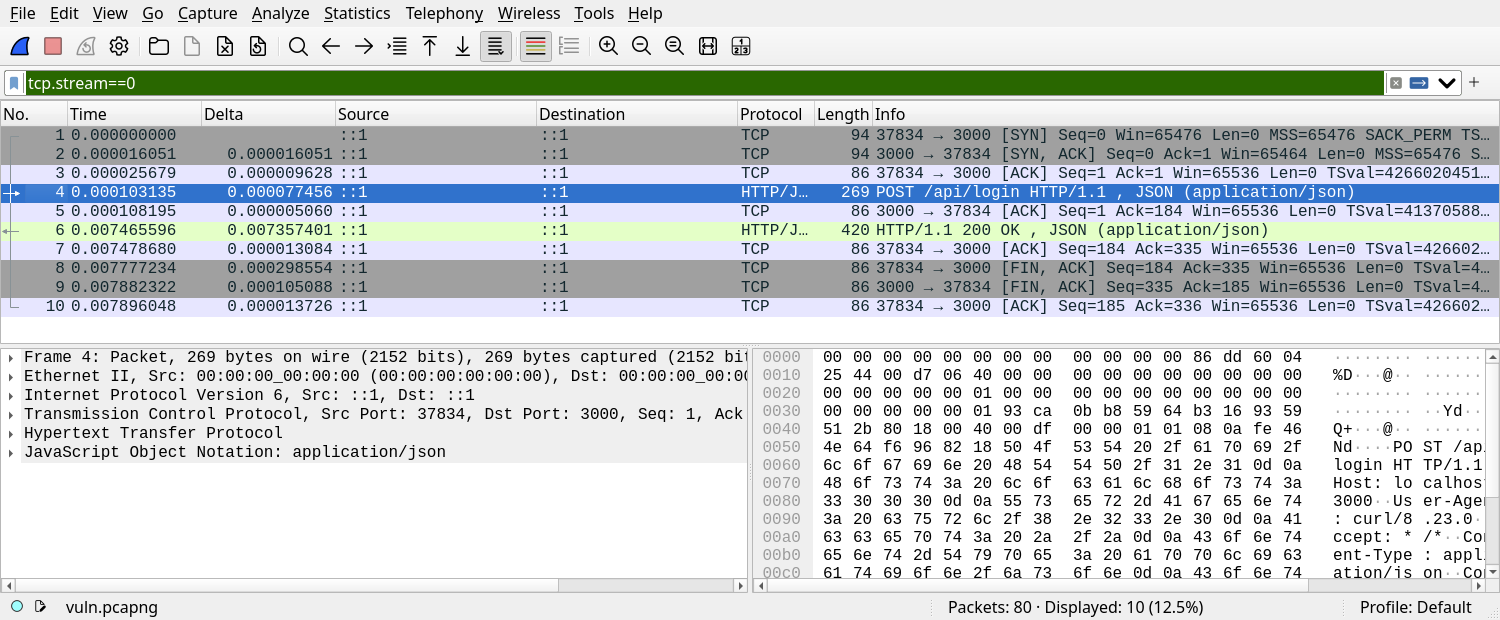
\includegraphics[width=\linewidth]{ws-vuln-list}
\caption{\vuln: połączenie logowania w~Wiresharku, zaznaczone \kod{POST /api/login}}\label{fig:wsv}\end{figure}
\begin{figure}[H]\centering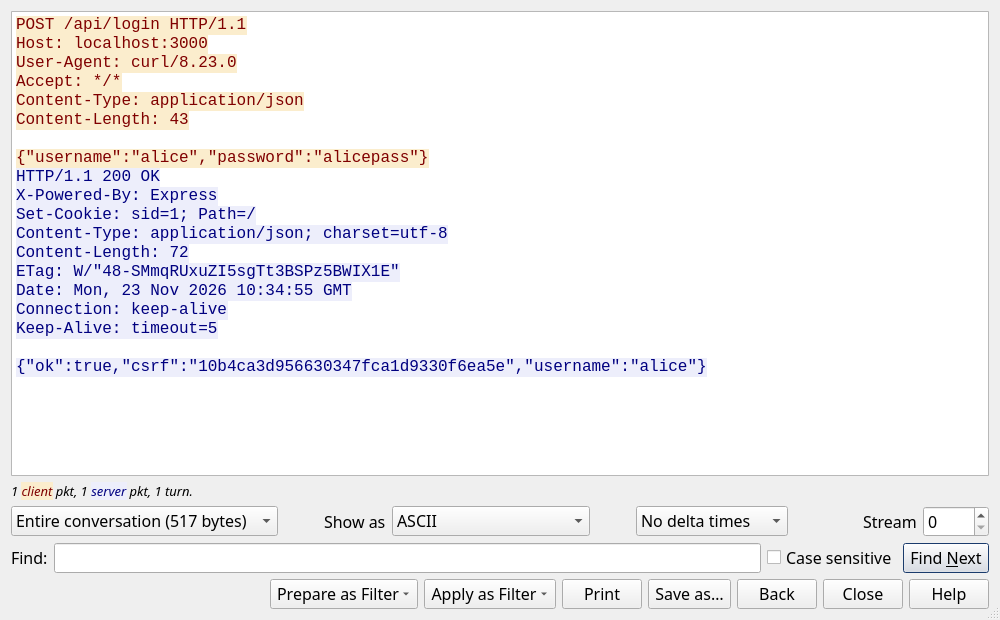
\includegraphics[width=.82\linewidth]{ws-vuln-follow}
\caption{\vuln: treść połączenia --- hasło i~cookie tekstem jawnym}\label{fig:wsvf}\end{figure}

Podsłuch wystarcza do przejęcia konta bez znajomości hasła. Cookie odczytane z~pliku \kod{vuln.pcapng} wysłano ponownie, gdy sesja była aktywna:
\dowod{replay.txt}{Odtworzenie sesji z przechwyconego cookie}

\subsection{Tryb zabezpieczony}
Widoczne są tylko rekordy TLS (rys.~\ref{fig:wss}), a~treść połączenia jest nieczytelna (rys.~\ref{fig:wssf}). We wszystkich ośmiu połączeniach wynegocjowano TLS~1.3, szyfr \kod{TLS\_AES\_256\_GCM\_SHA384} i~grupę X25519MLKEM768 (numer 4588), czyli hybrydową wymianę klucza odporną na atak „przechwyć teraz, odszyfruj później”. Wybór ten wynika z~domyślnych ustawień OpenSSL po obu stronach; serwer akceptuje również TLS~1.2.

\begin{figure}[H]\centering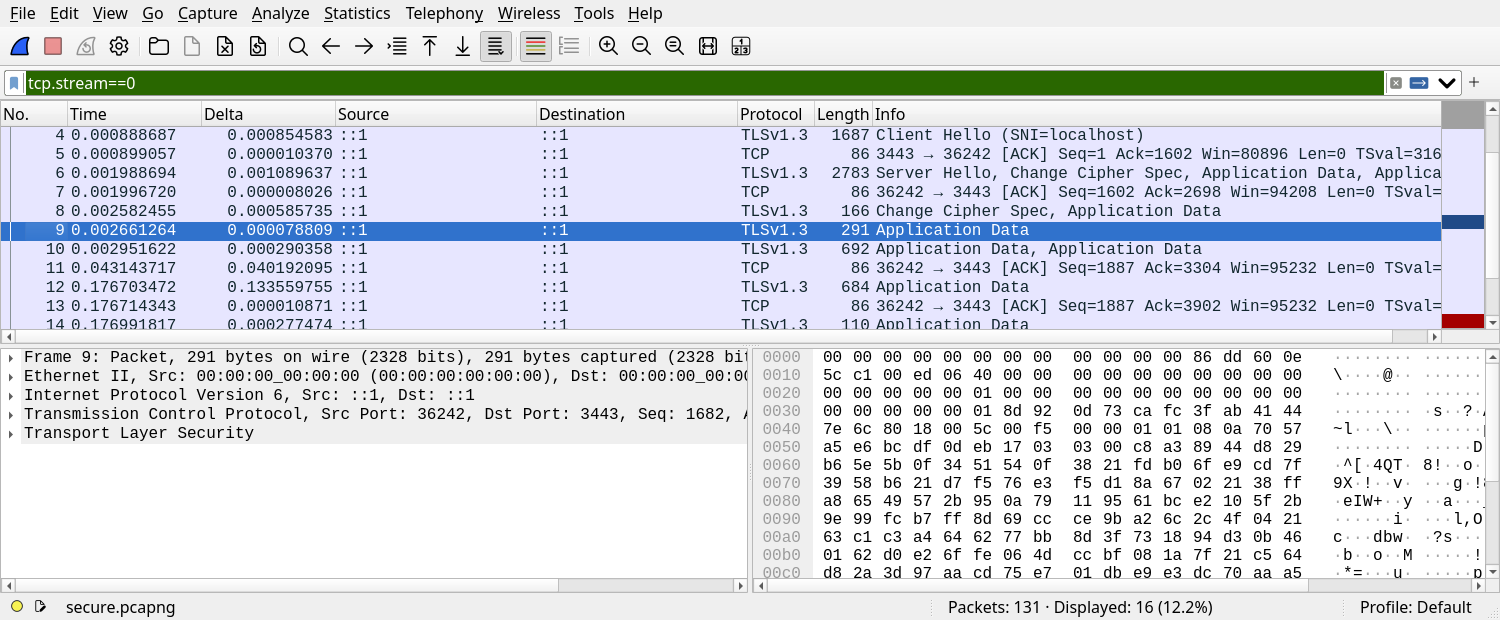
\includegraphics[width=\linewidth]{ws-secure-list}
\caption{\secure: to samo logowanie; żądanie HTTP jest w~ramce 9 jako \kod{Application Data}}\label{fig:wss}\end{figure}
\begin{figure}[H]\centering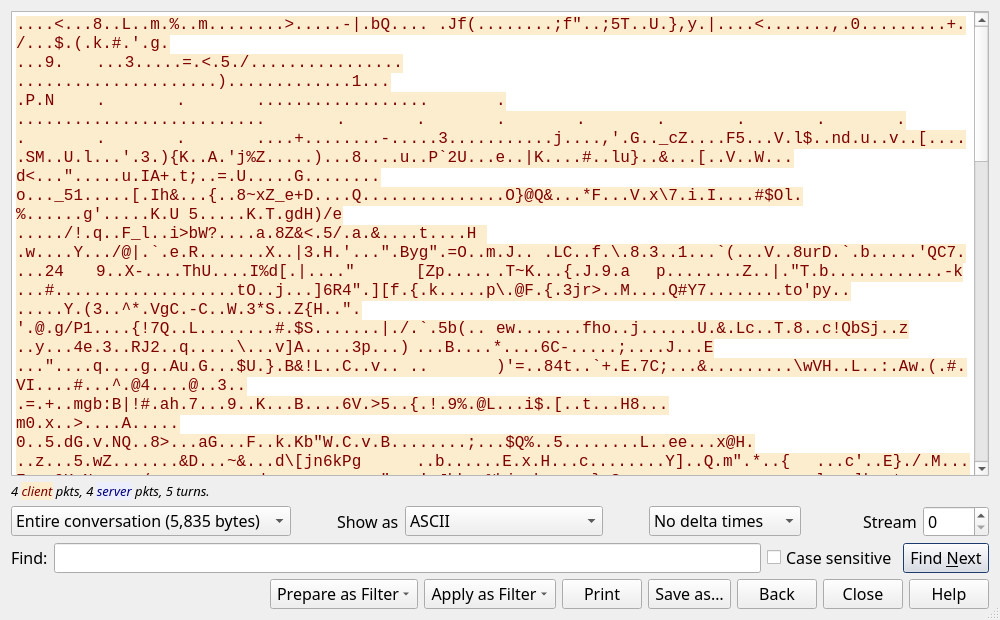
\includegraphics[width=.82\linewidth]{ws-secure-follow}
\caption{\secure: treść połączenia}\label{fig:wssf}\end{figure}

\begin{table}[H]\centering\caption{Liczba ramek zawierających dany ciąg}\label{tab:str}
\begin{tabular}{lrr}
\toprule
Szukany ciąg & \vuln & \secure\\\midrule
\kod{alicepass} (hasło) & 1 & 0\\
\kod{PIN do karty} (treść notatki) & 4 & 0\\
\kod{csrf} & 2 & 0\\
\kod{Cookie} & 8 & 0\\
\kod{/api/notes} (adresy) & 6 & 0\\
\kod{localhost} & 8 & 8\\
\bottomrule
\end{tabular}
\end{table}
Nazwa \kod{localhost} jest widoczna także w~\secure, ponieważ pole SNI w~\kod{ClientHello} nie jest szyfrowane. Certyfikat serwera w~TLS~1.3 jest już przesyłany w~postaci zaszyfrowanej.

Aby upewnić się, że wewnątrz jest ten sam protokół, ten sam plik odczytano z~kluczami sesji zapisanymi przez klienta (\kod{SSLKEYLOGFILE}). Bez kluczy, które nigdy nie są przesyłane siecią, odczyt jest niemożliwy:
\dowod{secure-login-decrypted.txt}{secure.pcapng odczytany z kluczami sesji}

\subsection{Co widać mimo szyfrowania}
Podsłuchujący nadal zna adresy, porty, nazwę serwera, chwile i~rozmiary. W~TLS~1.3 z~AES-GCM rekord jest dłuższy od danych o~stałe 17~bajtów (1~B typu treści i~16~B znacznika uwierzytelniającego), więc długość żądania HTTP można odczytać co do bajta (tab.~\ref{tab:rozm}).

\begin{table}[H]\centering\caption{Długość żądania HTTP i~rekordu TLS, który je przenosi (\secure)}\label{tab:rozm}
\small
\begin{tabular}{lrrr@{\hskip 3mm}lrrr}
\toprule
Operacja & HTTP [B] & TLS [B] & różnica & Operacja & HTTP [B] & TLS [B] & różnica\\\midrule
logowanie & 183 & 200 & 17 & edycja & 318 & 335 & 17\\
lista & 204 & 221 & 17 & wyszukiwanie & 212 & 229 & 17\\
utworzenie & 317 & 334 & 17 & usunięcie & 257 & 274 & 17\\
odczyt & 206 & 223 & 17 & sesja & 201 & 218 & 17\\
\bottomrule
\end{tabular}
\end{table}
W~badanym scenariuszu wszystkie osiem długości jest różnych, więc sama długość pozwala rozpoznać operację. Logowanie zdradza też czas: odpowiedź nadeszła po ok.~174~ms (koszt scrypt), podczas gdy pozostałe operacje trwają znacznie krócej. Jest to praktyczny przykład kanału bocznego opisanego przez Chena i~in.~\cite{chen}.

\subsection{Koszt zabezpieczeń}
\begin{table}[H]\centering\caption{Ruch na operację: ramki i~bajty na łączu}\label{tab:ops}
\begin{tabular}{lrrrr}
\toprule
& \multicolumn{2}{c}{\vuln} & \multicolumn{2}{c}{\secure}\\
Operacja & ramki & bajty & ramki & bajty\\\midrule
logowanie & 10 & 1393 & 16 & 7227\\
lista & 10 & 1364 & 16 & 7137\\
utworzenie & 10 & 1364 & 18 & 7297\\
odczyt & 10 & 1298 & 16 & 7071\\
edycja & 10 & 1369 & 17 & 7228\\
wyszukiwanie & 10 & 1306 & 16 & 7079\\
usunięcie & 10 & 1308 & 16 & 7081\\
sesja & 10 & 1304 & 16 & 7077\\\midrule
razem & 80 & 10\,706 & 131 & 57\,197\\
\bottomrule
\end{tabular}
\end{table}
Ruch w~\secure{} jest 5{,}3 raza większy, ale jest to przypadek najgorszy: każda operacja w~nowym połączeniu, z~pełnym uzgadnianiem. Dominuje stały koszt uzgodnienia. Sam udział klucza X25519MLKEM768 to 1216~B od klienta i~1120~B od serwera. Przeglądarka utrzymuje połączenie (keep-alive), więc ponosi ten koszt raz.

\begin{table}[H]\centering\caption{Średni czas odpowiedzi (pętla zwrotna)}\label{tab:czas}
\begin{tabular}{lrr}
\toprule
Pomiar & \vuln{} [ms] & \secure{} [ms]\\\midrule
nowe połączenie ($n=200$) & 0{,}57 & 2{,}79\\
to samo połączenie ($n=199$) & 0{,}13 & 0{,}14\\
logowanie ($n=20$) & 0{,}86 & 172{,}69\\
\bottomrule
\end{tabular}
\end{table}
Uzgodnienie TLS kosztuje ok.~2{,}2~ms, a~w~utrzymywanym połączeniu różnica jest pomijalna. Na pętli zwrotnej opóźnienie sieci jest bliskie zeru; w~rzeczywistej sieci doszłoby jedno dodatkowe RTT na uzgodnienie. Logowanie jest wolniejsze o~ok.~170~ms celowo: to koszt, który ponosi też napastnik przy każdym odgadywanym haśle.

\section{Analiza bezpieczeństwa}

\begin{table}[H]\centering\footnotesize\caption{Podatności i~wyniki ataków (przyporządkowanie do kategorii własne)}\label{tab:podat}
\begin{tabularx}{\linewidth}{rL{3.3cm}llXX}
\toprule
Nr & Podatność & OWASP & CWE & Wynik w~\vuln & Wynik w~\secure\\\midrule
1 & Brak szyfrowania & A04 & 319 & hasło i~cookie czytelne & 0 ramek z~danymi\\
2 & SQL injection & A05 & 89 & logowanie bez hasła, zrzut kont & 401, pusta lista\\
3 & Trwały XSS & A05 & 79 & skrypt wykonany, cookie wysłane & zwykły tekst\\
4 & Hasła tekstem jawnym & A04 & 256 & \kod{alicepass} w~bazie & skrót scrypt\\
5 & IDOR & A01 & 639 & odczyt i~zmiana cudzej notatki & 404\\
6 & Atrybuty cookie & A02 & 614, 1004 & brak & komplet, \kod{\_\_Host-}\\
7 & CSRF & A01 & 352 & obca strona tworzy notatkę & 401 / 403\\
8 & Brak limitu logowań & A07 & 307 & hasło znalezione w~15.~próbie & 429 od 6.~próby\\
9 & Brak nagłówków & A02 & 693 & brak, \kod{X-Powered-By} & CSP, HSTS, XFO, nosniff\\
10 & Przewidywalna sesja & A07 & 340 & przejęcie przez \kod{sid=1} & 401\\
11 & Ślad stosu w~błędach & A10 & 209 & ścieżki i~nazwy plików & komunikat ogólny\\
\bottomrule
\end{tabularx}
\end{table}

\subsection{SQL injection i hasła (2, 4)}
Tautologia w~nazwie użytkownika omija sprawdzenie hasła, a~zapytanie UNION w~wyszukiwarce zwraca tabelę kont zamiast notatek. Ponieważ hasła są jawne, jedno zapytanie kończy się pełnym przejęciem kont. Skutek pokazuje, jak podatności się wzmacniają: przy skrótach scrypt ten sam zrzut nie dałby gotowych haseł.
\dowod{vuln-sqli.txt}{VULN: attacks/sqli.sh}
\dowod{secure-sqli.txt}{SECURE: attacks/sqli.sh}

\subsection{Trwały XSS (3, 6)}
Notatka o~treści \kod{<img src=x onerror=...>} w~\vuln{} wykonuje kod przy każdym wyświetleniu i~wysyła cookie na serwer napastnika (w~logu pojawiło się \kod{GET /steal?c=sid=1}). W~\secure{} ten sam zapis jest zwykłym tekstem (rys.~\ref{fig:xss}). Sprawdzono też samą politykę CSP: po wstrzyknięciu surowego HTML z~pominięciem \kod{textContent} skrypt nadal się nie wykonał, a~cookie z~\kod{HttpOnly} było niewidoczne dla \kod{document.cookie}.
\begin{figure}[H]\centering
\begin{minipage}[t]{.48\linewidth}\centering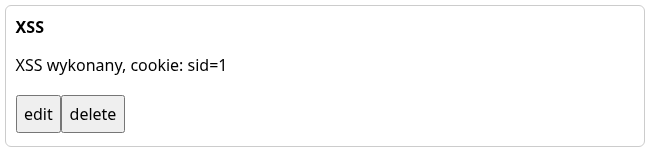
\includegraphics[width=\linewidth]{vuln-xss}\\\vuln\end{minipage}\hfill
\begin{minipage}[t]{.48\linewidth}\centering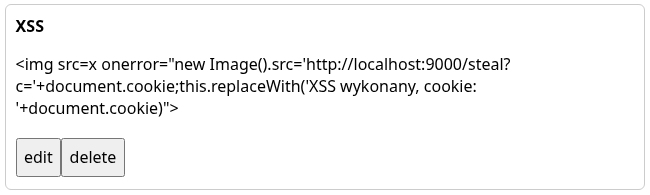
\includegraphics[width=\linewidth]{secure-xss}\\\secure\end{minipage}
\caption{Ta sama notatka w~obu trybach}\label{fig:xss}\end{figure}

\subsection{IDOR (5)}
Alicja, używając własnej sesji i~własnego tokenu CSRF, odczytuje i~nadpisuje notatkę Boba, zgadując jej numer:
\dowod{vuln-idor.txt}{VULN: attacks/idor.sh}
\dowod{secure-idor.txt}{SECURE: attacks/idor.sh}

\subsection{CSRF (7)}\label{sec:csrf}
Strona \kod{attacks/csrf.html} automatycznie wysyła ukryty formularz do aplikacji. Pierwsza wersja ataku używała \kod{fetch} z~metodą \kod{DELETE} i~nie działała: takie żądanie poprzedza zapytanie CORS \emph{preflight}, które przeglądarka odrzuciła. Formularz POST jest żądaniem prostym, więc nie podlega tej kontroli. Mechanizm CORS nie jest zatem ochroną przed CSRF.

\begin{table}[H]\centering\caption{CSRF w~zależności od przeglądarki i~pochodzenia strony}\label{tab:csrf}
\begin{tabularx}{\linewidth}{Xll}
\toprule
Scenariusz & Chrome 158 & Firefox 160\\\midrule
\vuln, strona z~\kod{localhost:9000} (ta sama witryna) & udany & udany\\
\vuln, strona z~\kod{127.0.0.1:9000}, świeże cookie & udany & udany\\
\vuln, strona z~\kod{127.0.0.1:9000}, cookie sprzed 130~s & zablokowany & udany\\
\secure, strona z~\kod{127.0.0.1:9000} & 401 & 401\\
\secure, strona z~\kod{http://localhost:9000} & 401 & \textbf{403}\\
\bottomrule
\end{tabularx}
\end{table}
Najciekawszy jest ostatni wiersz. Firefox wysłał cookie \kod{SameSite=Strict}, ponieważ domyślnie nie uwzględnia schematu (\kod{http}/\kod{https}) przy porównywaniu witryn; po włączeniu opcji \kod{network.cookie.sameSite.schemeful} odpowiedź zmieniła się na 401. Atak zatrzymał dopiero token CSRF (403). Chrome z~kolei traktuje cookie bez \kod{SameSite} jak \kod{Lax}, z~wyjątkiem pierwszych dwóch minut. Żaden z~mechanizmów sam nie wystarcza, co uzasadnia obronę warstwową.

\subsection{Logowanie i sesja (8, 10)}
Atak słownikowy w~\vuln{} znajduje hasło w~piętnastej próbie. W~\secure{} od szóstej próby serwer odpowiada 429 i~nie sprawdza haseł, więc poprawne hasło z~końca listy nie zostaje odkryte:
\begin{Verbatim}[label=attacks/bruteforce.sh (skrót)]
VULN    attempt 5 -> 401   attempt 6 -> 401   ...   attempt 15 (alicepass) -> 200
SECURE  attempt 5 -> 401   attempt 6 -> 429   ...   attempt 15 (alicepass) -> 429
\end{Verbatim}
Identyfikator sesji w~\vuln{} to kolejna liczba, więc wystarczy sprawdzić \kod{sid=1}:
\dowod{vuln-session.txt}{VULN: odgadywanie identyfikatora}
W~\secure{} token ma 256~bitów losowości, a~sesja wygasa po 30~minutach także po stronie serwera.

\subsection{Nagłówki i obsługa błędów (9, 11)}
\dowod{secure-headers.txt}{SECURE: nagłówki odpowiedzi}
Błędny JSON w~\vuln{} zwraca ślad stosu ze ścieżkami katalogów i~nazwami plików bibliotek (fragment):
\dowod[firstline=8,lastline=8]{vuln-error.txt}{VULN: odpowiedź na błędny JSON}
\dowod{secure-error.txt}{SECURE}

\section{Weryfikacja}
Polecenie \kod{npm test} uruchamia oba tryby na osobnych portach i~sprawdza oczekiwany wynik każdego ataku: w~\vuln{} atak musi się udać, w~\secure{} musi zawieść. Wszystkie 28 testów kończy się powodzeniem. Aby sprawdzić, czy testy wykrywają regresje, w~kopii projektu usuwano pojedyncze zabezpieczenia: kontrolę właściciela w~\kod{PUT}, \kod{HttpOnly}, token CSRF, limit logowań, wygasanie sesji i~obsługę błędów. W~każdym z~sześciu przypadków testy zgłosiły błąd.

Zachowania zależne od przeglądarki (XSS, CSRF, praca obu trybów obok siebie, operacje CRUD w~interfejsie) sprawdzono w~Chrome~158 i~Firefoksie~160, sterowanych skryptem w~trybie bez okna.

\section{Wdrożenie i instrukcja użytkownika}

\subsection{Instalacja}
Wymagania: Node.js w~wersji co najmniej 22.13 (testowano 26), \kod{mkcert}; do pomiarów także \kod{tshark}.
\begin{Verbatim}
npm install
mkcert -install
mkdir -p certs
mkcert -key-file certs/localhost-key.pem -cert-file certs/localhost.pem localhost 127.0.0.1
\end{Verbatim}

\subsection{Uruchomienie}
\begin{Verbatim}
npm run start:vuln      # http://localhost:3000
npm run start:secure    # https://localhost:3443
npm test                # testy obu trybów
report/collect.sh       # odtworzenie pomiarów z rozdziału 6
\end{Verbatim}
Oba tryby mogą działać jednocześnie. Ponowne uruchomienie przywraca dane początkowe. Konta demonstracyjne: \kod{alice}/\kod{alicepass}, \kod{bob}/\kod{bobsecret}.

\subsection{Obsługa aplikacji}
\begin{enumerate}
\item \textbf{Rejestracja}: wpisać nazwę i~hasło, wybrać \emph{Register}. W~\secure{} nazwa ma 3--32 znaki (litery, cyfry, \kod{\_ . -}), a~hasło co najmniej 8.
\item \textbf{Logowanie}: \emph{Log in}. Po pięciu nieudanych próbach w~\secure{} należy odczekać minutę.
\item \textbf{Dodanie notatki}: wypełnić \emph{title} i~\emph{body}, wybrać \emph{Add note}.
\item \textbf{Edycja}: \emph{edit} przy notatce przenosi jej treść do formularza; \emph{Save} zapisuje, \emph{Cancel} porzuca zmiany (rys.~\ref{fig:edit}).
\item \textbf{Usunięcie}: \emph{delete} przy notatce.
\item \textbf{Wyszukiwanie}: pole na górze filtruje po tytule.
\item \textbf{Wylogowanie}: \emph{Log out}. Odświeżenie strony nie wylogowuje.
\end{enumerate}
\begin{figure}[H]\centering
\begin{minipage}[t]{.48\linewidth}\centering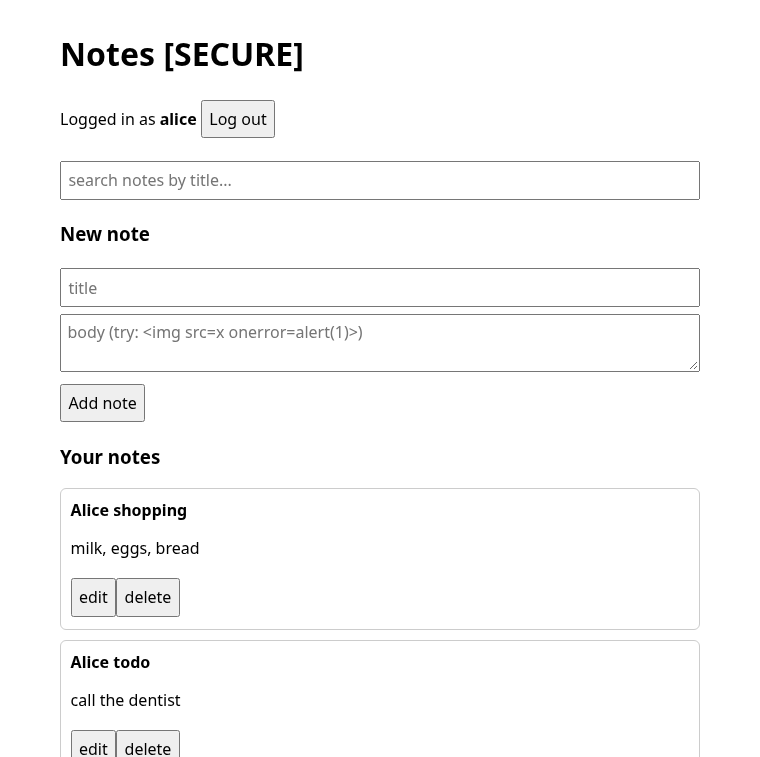
\includegraphics[width=\linewidth]{secure-notes}\end{minipage}\hfill
\begin{minipage}[t]{.48\linewidth}\centering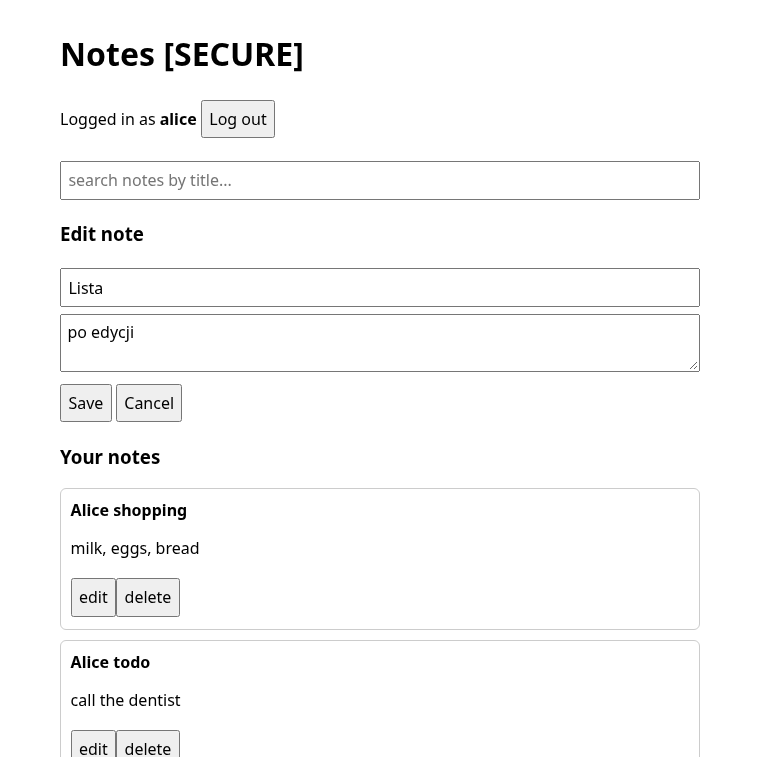
\includegraphics[width=\linewidth]{secure-edit}\end{minipage}
\caption{Lista notatek i~edycja}\label{fig:edit}\end{figure}

\section{Ograniczenia i możliwości rozwoju}
\begin{itemize}
\item \textbf{Hasła}: minimum 8 znaków spełnia ASVS, ale nie NIST (15 znaków przy jednym składniku). Dalsze kroki: 15 znaków, sprawdzanie na listach wycieków, Argon2id, drugi składnik lub klucze dostępu (passkeys).
\item \textbf{Limit logowań}: liczony na adres IP i~w~pamięci procesu. Atak rozproszony go omija; potrzebny jest dodatkowy limit na konto i~wspólny magazyn.
\item \textbf{Wydajność}: \kod{scryptSync} blokuje pętlę zdarzeń na czas logowania; przy większym ruchu należy użyć wersji asynchronicznej.
\item \textbf{Ujawnianie kont}: rejestracja nadal zdradza zajętą nazwę (409).
\item \textbf{Sesje}: jest limit bezwzględny, brak limitu bezczynności; sesje giną po restarcie.
\item \textbf{CSP}: można dodać \kod{frame-ancestors}, \kod{base-uri}, \kod{form-action} i~Trusted Types.
\item \textbf{Rejestrowanie zdarzeń} (A09): brak dziennika nieudanych logowań i~alarmów.
\item \textbf{Transmisja}: przekierowanie z~HTTP, certyfikat publicznego CA (ACME), wymuszenie TLS~1.3, Encrypted Client Hello (ukrycie SNI), dopełnianie rekordów utrudniające analizę rozmiarów.
\item \textbf{Proces}: \kod{npm test} i~\kod{npm audit} w~CI, skanowanie dynamiczne (np. OWASP ZAP), trwała baza.
\item \textbf{Badania}: porównanie z~HTTP/3 oraz pomiar w~sieci o~rzeczywistym opóźnieniu.
\end{itemize}

\section{Podsumowanie}
Zbudowano aplikację CRUD, której dwa tryby różnią się wyłącznie zabezpieczeniami. W~trybie niezabezpieczonym podsłuch jednego połączenia ujawnia hasło i~pozwala przejąć sesję, a~wszystkie jedenaście podatności udało się zademonstrować. W~trybie zabezpieczonym te same ataki zawiodły, a~w~ruchu nie znaleziono ani jednej ramki z~hasłem, cookie czy treścią notatki.

Najważniejsze wnioski: (1)~TLS chroni treść, ale nie rozmiary i~czasy, które pozwoliły rozpoznać wykonywane operacje; (2)~szyfrowanie transmisji nie chroni przed błędami aplikacji, takimi jak SQL injection czy IDOR; (3)~zachowanie przeglądarek różni się na tyle, że pojedyncze zabezpieczenie bywa niewystarczające, co pokazał test CSRF w~Firefoksie; (4)~koszt TLS przy utrzymywanym połączeniu jest pomijalny.

\begin{thebibliography}{99}\small
\bibitem{owasptop10} OWASP, \emph{OWASP Top 10:2025}. \url{https://top10.owasp.org/2025/0x00_2025-Introduction} (dostęp 23.11.2026).
\bibitem{asvs} OWASP, \emph{Application Security Verification Standard 5.0}, wymaganie 6.2.1. \url{https://github.com/OWASP/ASVS}.
\bibitem{saltzer} J. H. Saltzer, M. D. Schroeder, \emph{The Protection of Information in Computer Systems}, Proceedings of the IEEE 63(9), 1975, s.~1278--1308. doi:10.1109/PROC.1975.9939.
\bibitem{deroo} R. De Roo, \emph{Teaching Web Security Through Vulnerabilities: A Comparative Study of Vulnerable Web Applications}, praca licencjacka, Royal Military Academy, Bruksela 2026. \url{https://cylab.be/publications/92}.
\bibitem{gruyere} Y. Ni, Z. Li, X. Li, \emph{Security Analysis of Web Applications Based on Gruyere}, arXiv:2509.14706, 2025.
\bibitem{halfond} W. G. J. Halfond, J. Viegas, A. Orso, \emph{A Classification of SQL Injection Attacks and Countermeasures}, ISSSE 2006.
\bibitem{csp} L. Weichselbaum, M. Spagnuolo, S. Lekies, A. Janc, \emph{CSP Is Dead, Long Live CSP!}, ACM CCS 2016, s.~1376--1387. doi:10.1145/2976749.2978363.
\bibitem{barth} A. Barth, C. Jackson, J. C. Mitchell, \emph{Robust Defenses for Cross-Site Request Forgery}, ACM CCS 2008, s.~75--88. doi:10.1145/1455770.1455782.
\bibitem{rfc6265} A. Barth, \emph{HTTP State Management Mechanism}, RFC 6265, 2011.
\bibitem{rfc6265bis} \emph{Cookies: HTTP State Management Mechanism}, draft-ietf-httpbis-rfc6265bis-22, IETF, grudzień 2025.
\bibitem{owaspsession} OWASP, \emph{Session Management Cheat Sheet}. \url{https://cheatsheetseries.owasp.org/cheatsheets/Session_Management_Cheat_Sheet.html} (dostęp 23.11.2026).
\bibitem{owasppass} OWASP, \emph{Password Storage Cheat Sheet}. \url{https://cheatsheetseries.owasp.org/cheatsheets/Password_Storage_Cheat_Sheet.html} (dostęp 23.11.2026).
\bibitem{rfc7914} C. Percival, S. Josefsson, \emph{The scrypt Password-Based Key Derivation Function}, RFC 7914, 2016.
\bibitem{nist} NIST, \emph{SP 800-63B-4}, 2025. \url{https://pages.nist.gov/800-63-4/sp800-63b.html}.
\bibitem{rfc9846} E. Rescorla, \emph{The Transport Layer Security (TLS) Protocol Version 1.3}, RFC 9846, 2026.
\bibitem{rfc6797} J. Hodges, C. Jackson, A. Barth, \emph{HTTP Strict Transport Security (HSTS)}, RFC 6797, 2012.
\bibitem{rfc10024} K. Kwiatkowski, P. Kampanakis, B. E. Westerbaan, D. Stebila, \emph{Post-Quantum Traditional (PQ/T) Hybrid Key Agreement Mechanisms for TLS 1.3}, RFC 10024, 2026.
\bibitem{chen} S. Chen, R. Wang, X. Wang, K. Zhang, \emph{Side-Channel Leaks in Web Applications: a Reality Today, a Challenge Tomorrow}, IEEE S\&P 2010, s.~191--206. doi:10.1109/SP.2010.20.
\end{thebibliography}
\end{document}
